% =====================================================================
%  SLIDE THUYẾT TRÌNH — HỆ THỐNG BÃI ĐỖ XE THÔNG MINH (INT3108)
%  Biên dịch tại thư mục report/slides/:
%     xelatex slides.tex      hoặc      tectonic slides.tex
%  Ảnh và sơ đồ dùng chung với báo cáo (../photos, ../diagrams).
% =====================================================================
\documentclass[aspectratio=169,11pt]{beamer}

\usepackage{fontspec}
\setsansfont{texgyreheros}[Extension=.otf,UprightFont=*-regular,
  BoldFont=*-bold,ItalicFont=*-italic,BoldItalicFont=*-bolditalic]
\setmonofont{texgyrecursor}[Extension=.otf,UprightFont=*-regular,
  BoldFont=*-bold,ItalicFont=*-italic,BoldItalicFont=*-bolditalic]
\usepackage[vietnamese,shorthands=off]{babel}
\usepackage{booktabs,tabularx,array}
\usepackage{tikz}
\usetikzlibrary{positioning,arrows.meta}
\graphicspath{{../}{../photos/}{../diagrams/}}

% ---------- Giao diện ----------
\definecolor{uet}{RGB}{0,62,126}
\definecolor{ok}{RGB}{46,125,50}
\definecolor{warn}{RGB}{199,119,0}
\definecolor{bad}{RGB}{198,40,40}
\definecolor{soft}{RGB}{238,243,250}
\usetheme{default}
\setbeamercolor{frametitle}{fg=white,bg=uet}
\setbeamercolor{structure}{fg=uet}
\setbeamercolor{block title}{fg=white,bg=uet}
\setbeamercolor{block body}{bg=soft}
\setbeamerfont{frametitle}{size=\large,series=\bfseries}
\setbeamertemplate{navigation symbols}{}
\setbeamertemplate{itemize items}[circle]
\setbeamertemplate{blocks}[rounded][shadow=false]
\setbeamertemplate{frametitle}{%
  \nointerlineskip
  \begin{beamercolorbox}[wd=\paperwidth,ht=2.6ex,dp=1.2ex,leftskip=1.2em]{frametitle}
    \usebeamerfont{frametitle}\insertframetitle
  \end{beamercolorbox}}
\setbeamertemplate{footline}{%
  \hbox{\begin{beamercolorbox}[wd=\paperwidth,ht=2.4ex,dp=1ex,leftskip=1.2em,rightskip=1.2em]{}%
    \tiny\color{gray}INT3108 · Bãi đỗ xe thông minh\hfill\insertframenumber/\inserttotalframenumber
  \end{beamercolorbox}}}
\newcommand{\code}[1]{\texttt{#1}}
\newcommand{\bt}[1]{\rule[-0.7ex]{0pt}{3.1ex}#1}
\newcommand{\pill}[2]{\tikz[baseline=(t.base)]\node[fill=#1,text=white,rounded corners=2pt,
  inner sep=2pt,font=\scriptsize\bfseries](t){#2};}

\title{Hệ thống bãi đỗ xe thông minh}
\subtitle{ESP32-C3 + ESP8266 · FreeRTOS · RFID · VietQR}
\date{Lập trình nhúng (INT3108) · Trường ĐH Công nghệ, ĐHQGHN}

\begin{document}

% ---------------------------------------------------------------------
\begin{frame}[plain]
\begin{tikzpicture}[remember picture,overlay]
  \fill[uet] (current page.north west) rectangle ([yshift=-4.1cm]current page.north east);
  \node[anchor=north west,inner sep=0] at ([xshift=1cm,yshift=-0.7cm]current page.north west)
    {
\includegraphics[height=1.4cm]{uet_logo.png}};
  \node[anchor=north west,text=white,font=\LARGE\bfseries] at ([xshift=2.8cm,yshift=-0.75cm]current page.north west)
    {Hệ thống bãi đỗ xe thông minh};
  \node[anchor=north west,text=white!85!uet] at ([xshift=2.8cm,yshift=-1.7cm]current page.north west)
    {ESP32-C3 + ESP8266 · FreeRTOS · RFID · VietQR qua SePay};
  \node[anchor=north west,text=white!70!uet,font=\small] at ([xshift=2.8cm,yshift=-2.6cm]current page.north west)
    {Lập trình nhúng (INT3108 1) · GV: Trần Hoàng Việt};
  \node[anchor=south west,inner sep=0] at ([xshift=1cm,yshift=1.1cm]current page.south west) {%
    \begin{tabular}{@{}ll@{}}
      \multicolumn{2}{@{}l}{\small\color{uet}\textbf{Nhóm thực hiện}}\\[2pt]
      Nguyễn Chí Minh & 24020232 \\
      Đinh Đức Thịnh & 24020313 \\
      Nguyễn Việt Tiến & 24020322 \\
    \end{tabular}};
  \node[anchor=south east,inner sep=0] at ([xshift=-1cm,yshift=0.7cm]current page.south east)
    {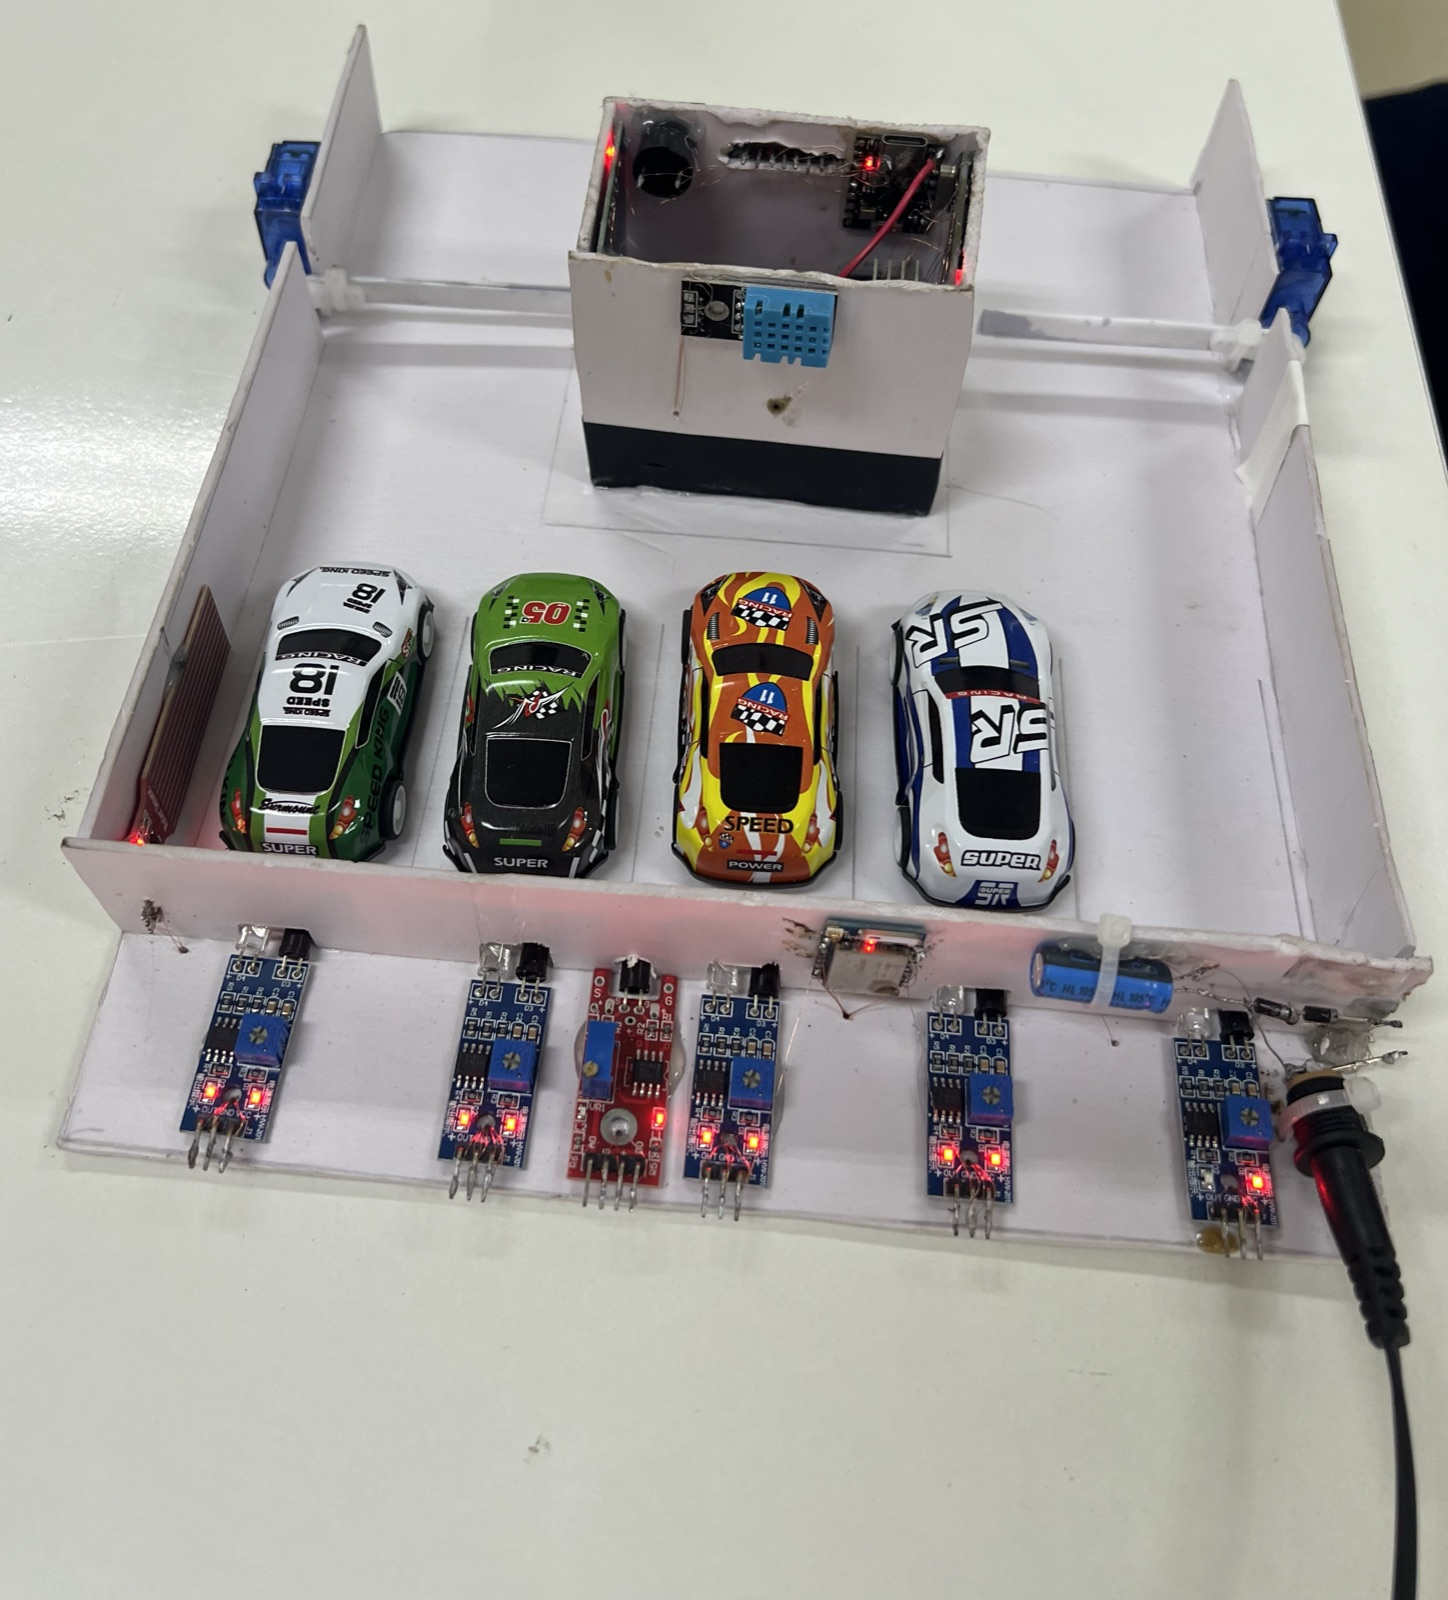
\includegraphics[height=4.6cm]{model_angle.jpg}};
\end{tikzpicture}
\end{frame}

% ---------------------------------------------------------------------
\begin{frame}{Nội dung}
\begin{columns}[T]
\column{0.48\textwidth}
\begin{enumerate}
  \item Bài toán và mục tiêu
  \item Mô hình thực tế
  \item Kiến trúc hệ thống và phần cứng
  \item Giao thức và phần mềm máy chủ
\end{enumerate}
\column{0.48\textwidth}
\begin{enumerate}\setcounter{enumi}{4}
  \item Chức năng: RFID, VietQR, an toàn, giám sát
  \item Kiểm thử
  \item \textbf{Demo trực tiếp}
  \item Kết luận và phân công
\end{enumerate}
\end{columns}
\end{frame}

% ---------------------------------------------------------------------
\begin{frame}{Bài toán và mục tiêu}
\begin{columns}[T]
\column{0.36\textwidth}
\begin{block}{\bt{Bãi xe thủ công hiện nay}}
\begin{itemize}\small
  \item Không biết trước còn chỗ trống
  \item Vé giấy, tính tiền bằng tay
  \item Không cảnh báo cháy, ngập ở tầng hầm
\end{itemize}
\end{block}
\vspace{4pt}
\small Mô hình: \textbf{5 chỗ đỗ, 2 cổng}, 3 bo mạch, linh kiện phổ thông giá rẻ.
\column{0.61\textwidth}
\footnotesize\renewcommand{\arraystretch}{1.25}
\begin{tabularx}{\linewidth}{@{}l>{\raggedright\arraybackslash}X@{}}
\toprule
\textbf{Mục tiêu} & \textbf{Cách đạt được} \\ \midrule
Chỗ trống thời gian thực & 5 cảm biến IR; TFT $\approx$ 0,1\,s, web $\approx$ 1\,s \\
Ra vào bằng thẻ & RFID MFRC522, servo tự đóng sau 3\,s \\
Tính phí tự động & 5.000\,đ/giờ, làm tròn lên, VietQR \\
An toàn & Cháy: còi + mở cả 2 cổng; ngập: khóa cổng vào \\
Giám sát từ xa & Web \code{parking.local}, không cần app \\
Triển khai đơn giản & 3 bo cùng vào một Wi-Fi chung \\
\bottomrule
\end{tabularx}
\end{columns}
\end{frame}

% ---------------------------------------------------------------------
\begin{frame}{Mô hình thực tế}
\centering
\begin{tabular}{@{}c@{\hspace{6pt}}c@{\hspace{6pt}}c@{}}
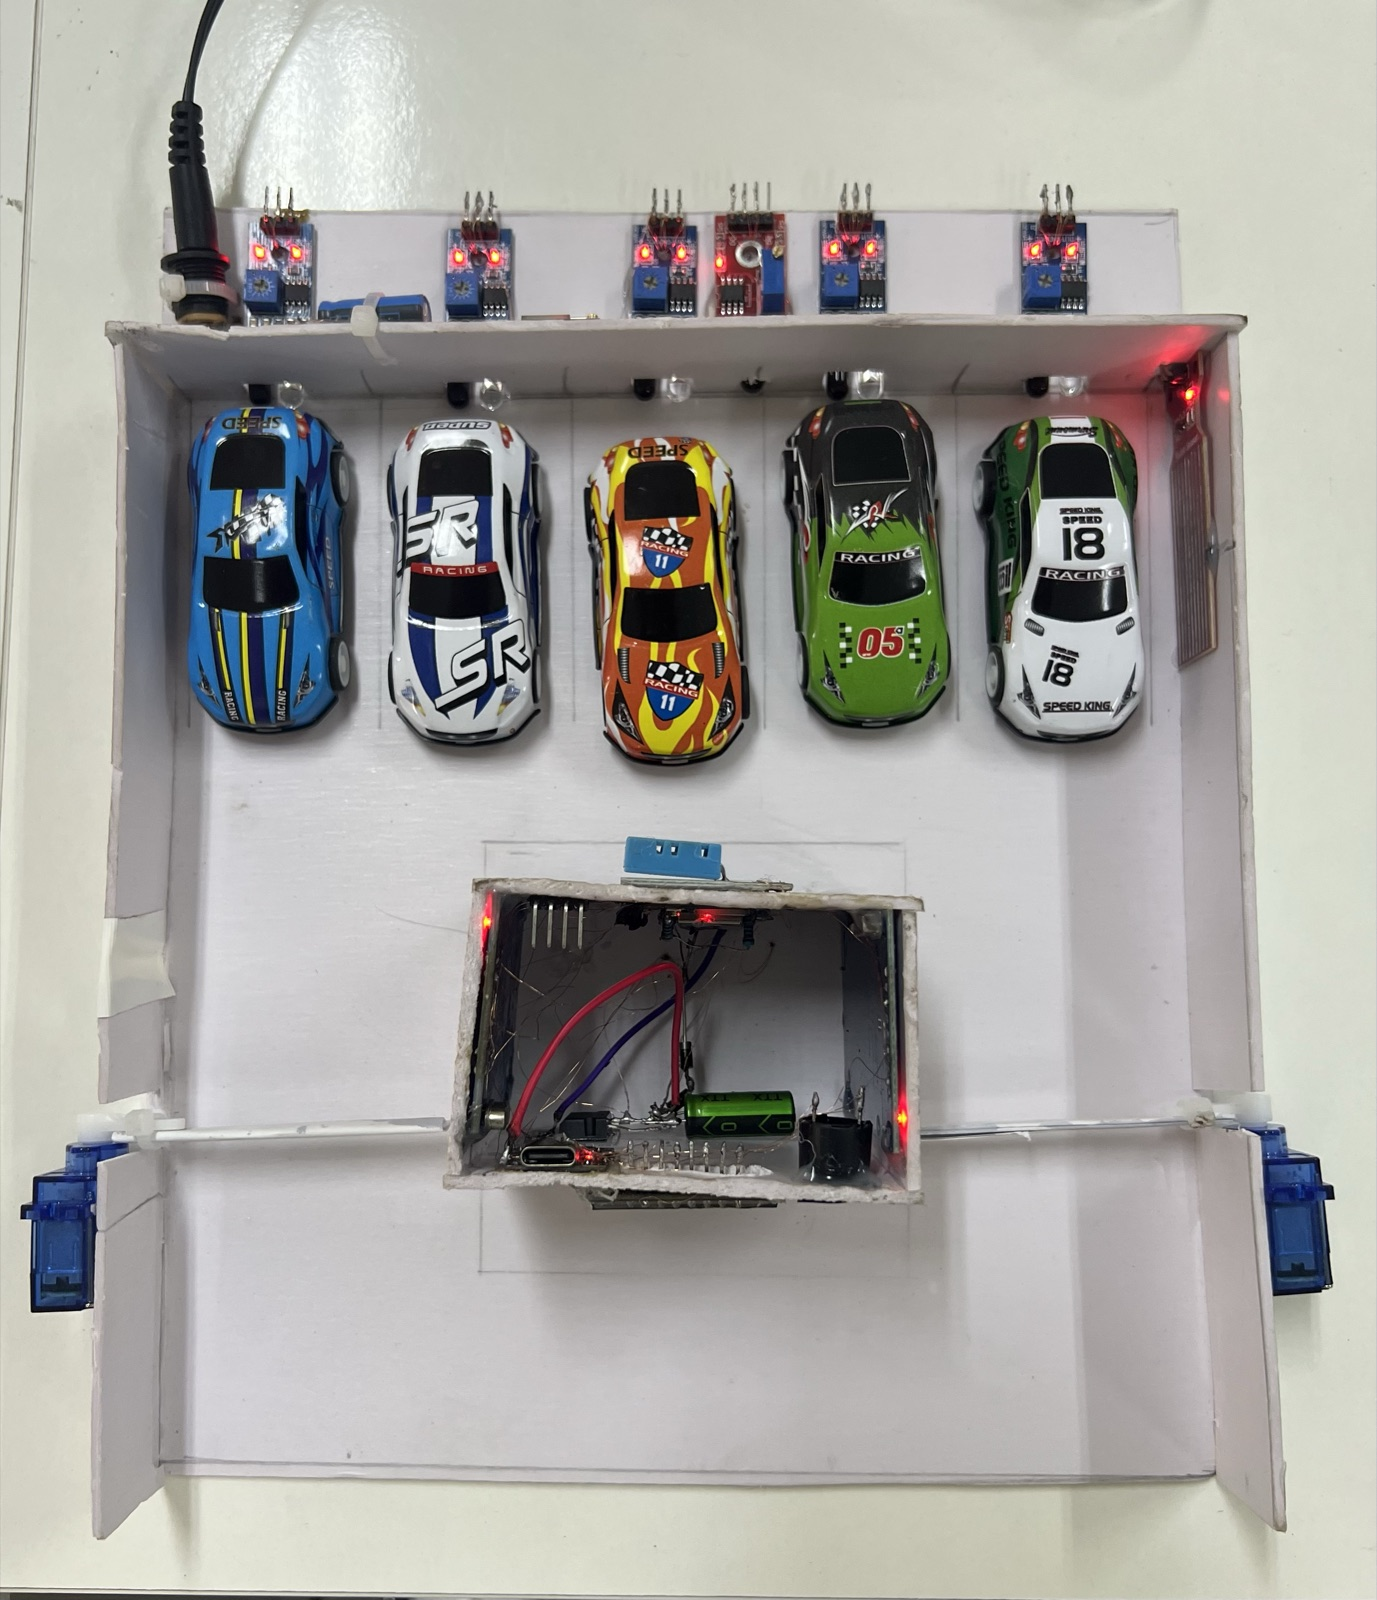
\includegraphics[height=5.4cm]{model_top.jpg} &
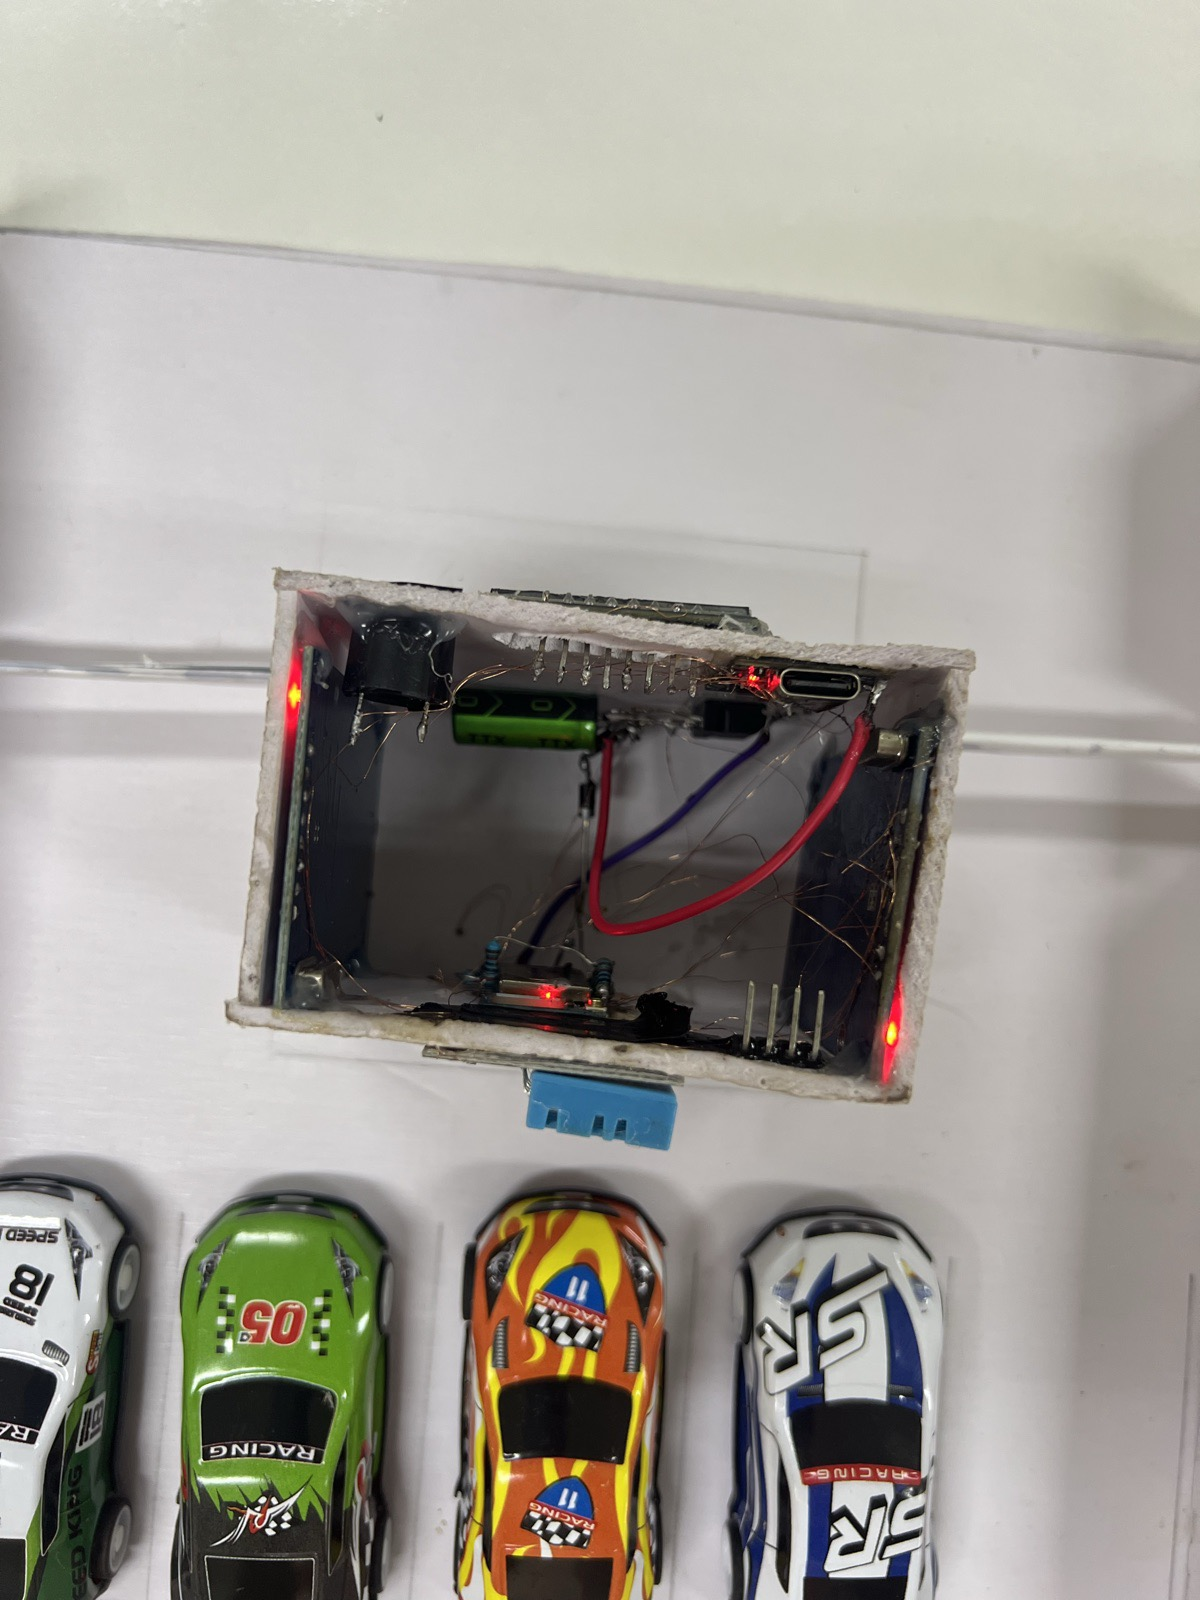
\includegraphics[height=5.4cm]{model_box.jpg} &
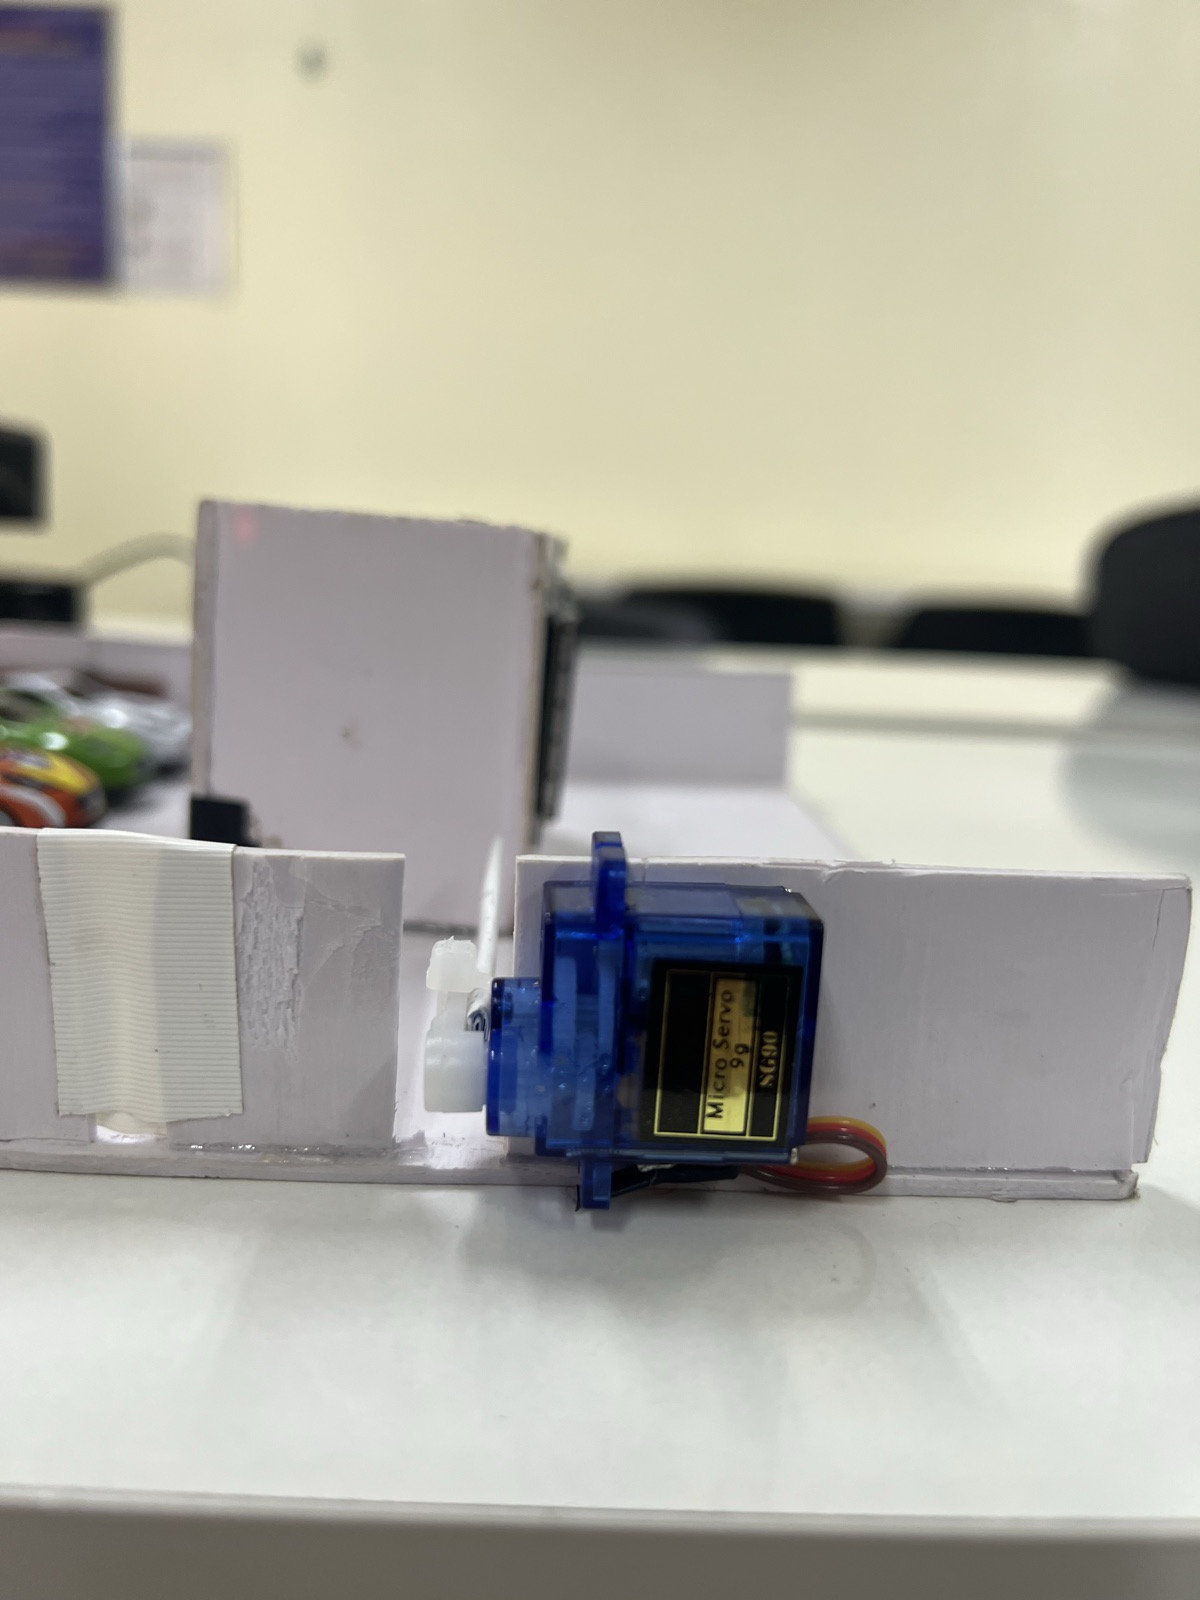
\includegraphics[height=5.4cm]{model_servo.jpg} \\[2pt]
\scriptsize Nhìn từ trên: 5 ô đỗ, 2 làn & \scriptsize Hộp mạch và nguồn & \scriptsize Thanh chắn servo SG90
\end{tabular}
\end{frame}

% ---------------------------------------------------------------------
\begin{frame}{Kiến trúc triển khai}
\begin{columns}[c]
\column{0.62\textwidth}
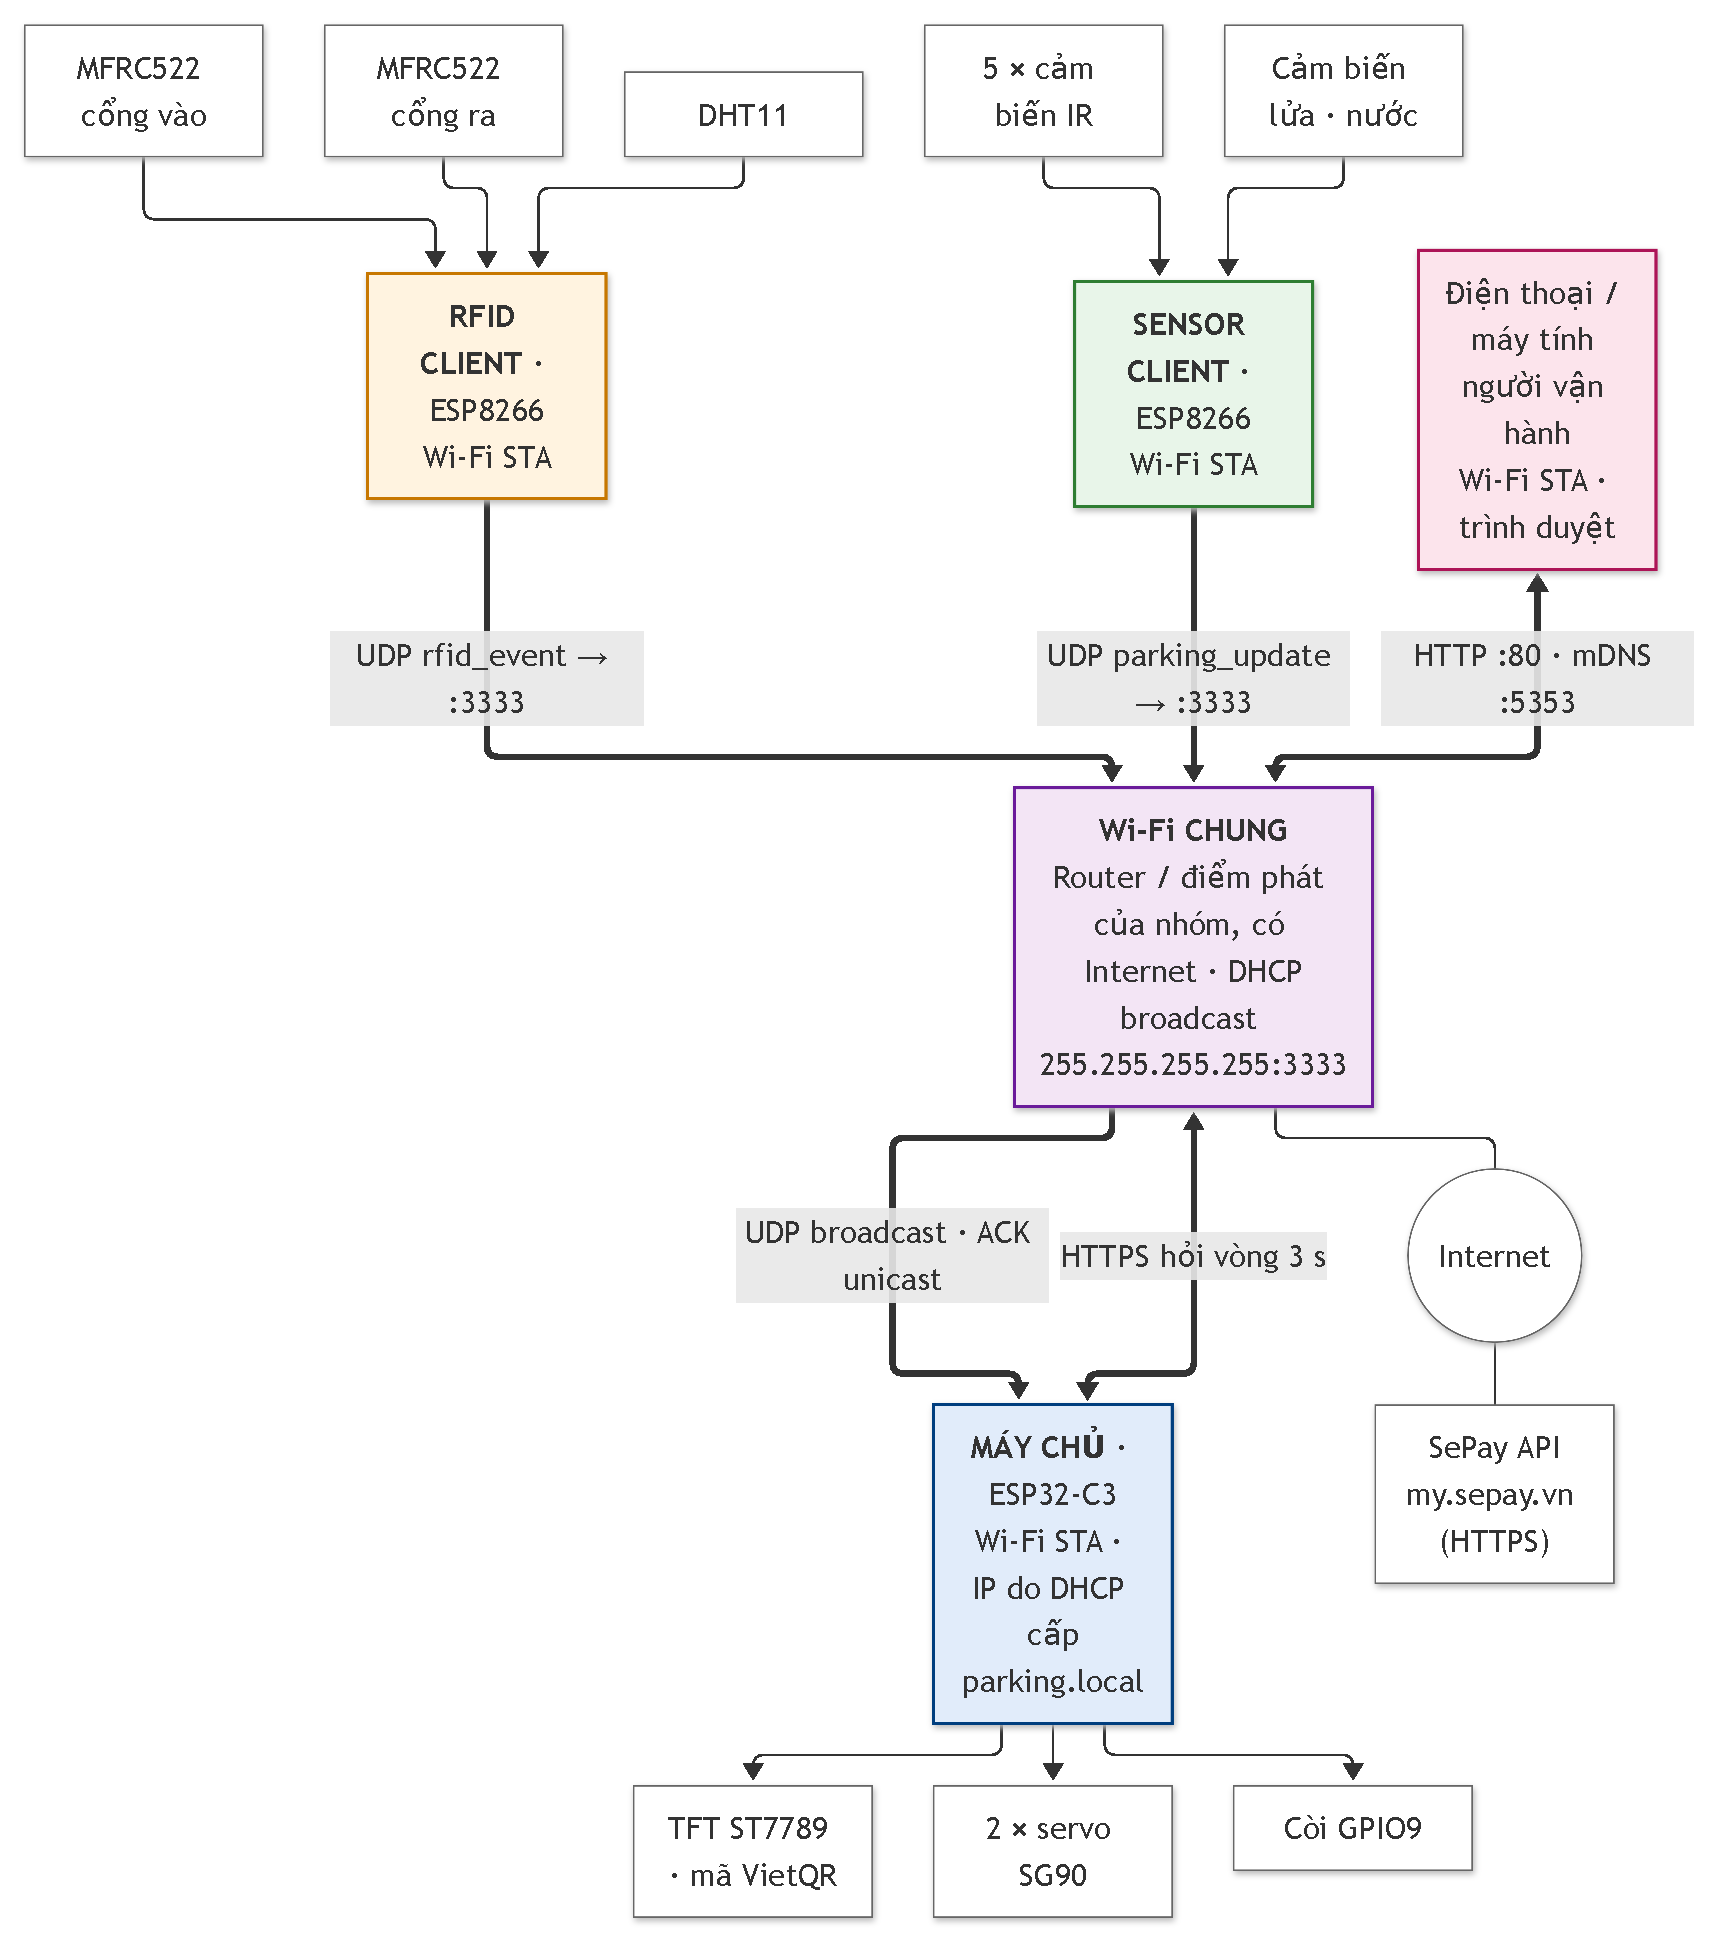
\includegraphics[width=\linewidth]{deploy.pdf}
\column{0.36\textwidth}
\small
\begin{itemize}
  \item Ba bo là \textbf{trạm Wi-Fi} trên mạng chung của nhóm, không bo nào phát Wi-Fi
  \item Client gửi \textbf{UDP broadcast} tới cổng 3333 — không cần biết IP máy chủ
  \item Máy chủ: web \code{:80}, tên \code{parking.local} qua mDNS
  \item Internet chỉ dùng để hỏi \textbf{SePay}; mất mạng thì bãi vẫn chạy
\end{itemize}
\end{columns}
\end{frame}

% ---------------------------------------------------------------------
\begin{frame}{Phần cứng: ba nút}
\small
\begin{tabularx}{\linewidth}{@{}l>{\raggedright\arraybackslash}X>{\raggedright\arraybackslash}X@{}}
\toprule
\textbf{Nút} & \textbf{Thiết bị} & \textbf{Nhiệm vụ} \\ \midrule
\textbf{Máy chủ} ESP32-C3 & TFT ST7789 240×240, 2 servo SG90, còi &
  Phiên RFID, tính phí, VietQR + SePay, thanh chắn, web, mDNS \\[3pt]
\textbf{Sensor Client} ESP8266 & 5 IR, cảm biến lửa, mực nước &
  Lọc nhiễu, gửi trạng thái mỗi 1\,s \\[3pt]
\textbf{RFID Client} ESP8266 & 2 MFRC522 (vào/ra), DHT11 &
  Gửi sự kiện quẹt thẻ, nhiệt độ mỗi 5\,s \\
\bottomrule
\end{tabularx}
\vspace{8pt}
\begin{block}{\bt{Vì sao chọn ESP32-C3 cho máy chủ?}}
Ảnh màn hình đã cần $240\times240\times2 = 115.200$\,B RAM — lớn hơn toàn bộ RAM của ESP8266.
ESP32-C3 có 400\,KB SRAM, SPI có DMA, PWM LEDC 14 bit và FreeRTOS chính thức.
\end{block}
\end{frame}

% ---------------------------------------------------------------------
\begin{frame}[fragile]{Giao thức UDP: JSON + ACK}
\begin{columns}[T]
\column{0.52\textwidth}
\small Bản tin JSON gọn, dễ gỡ lỗi:
\begin{block}{}
\scriptsize
\begin{verbatim}
{"type":"parking_update",
 "slots":[1,0,0,1,0],
 "water_mm":0.2,"fire":false}

{"type":"rfid_event","card_id":"A1B2C3D4",
 "gate":"in","temperature_c":28.5,
 "seq":91827}

{"type":"rfid_ack","seq":91827}
\end{verbatim}
\end{block}
\column{0.45\textwidth}
\small
\begin{itemize}
  \item UDP có thể mất gói $\Rightarrow$ quẹt thẻ cần \textbf{ACK}
  \item Chưa có ACK: gửi lại sau 300\,ms, tối đa 6 lần
  \item Máy chủ nhớ 16 \code{seq} gần nhất: gói lặp vẫn được ACK nhưng \textbf{chỉ xử lý một lần}
  \item Cảm biến gửi mỗi giây nên mất một gói cũng không sao
  \item Bộ đọc JSON không cấp phát động, kiểm tra mọi trường
\end{itemize}
\end{columns}
\end{frame}

% ---------------------------------------------------------------------
\begin{frame}{Phần mềm máy chủ: tác vụ FreeRTOS}
\begin{columns}[c]
\column{0.5\textwidth}
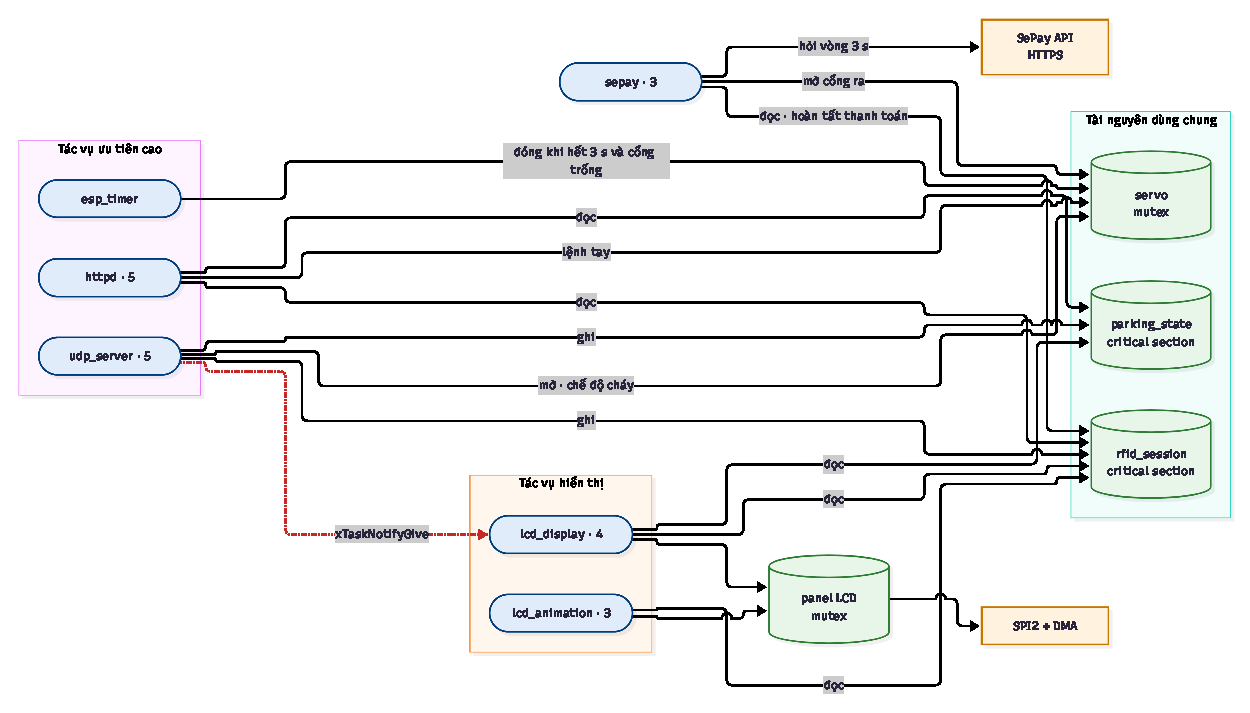
\includegraphics[width=\linewidth]{tasks.pdf}
\column{0.48\textwidth}
\scriptsize
\begin{tabularx}{\linewidth}{@{}lc>{\raggedright\arraybackslash}X@{}}
\toprule
\textbf{Tác vụ} & \textbf{Ưu tiên} & \textbf{Nhiệm vụ} \\ \midrule
\code{udp\_server} & 5 & Nhận bản tin, ra lệnh servo, còi, màn hình \\
\code{httpd} & 5 & Trang web và API \\
\code{lcd\_display} & 4 & Vẽ lại khi dữ liệu đổi \\
\code{lcd\_animation} & 3 & Ảnh động, 100\,ms/khung \\
\code{sepay} & 3 & Hỏi SePay qua HTTPS \\
\code{mdns} & 1 & Trả lời \code{parking.local} \\
\bottomrule
\end{tabularx}
\vspace{4pt}
\begin{itemize}
  \item Trạng thái dùng chung được bảo vệ bằng mutex
  \item Màn hình được đánh thức bằng task notification, không hỏi vòng
  \item Đóng thanh chắn bằng \code{esp\_timer}, chính xác tới micro giây
\end{itemize}
\end{columns}
\end{frame}

% ---------------------------------------------------------------------
\begin{frame}{Xe vào và ra bằng thẻ RFID}
\centering
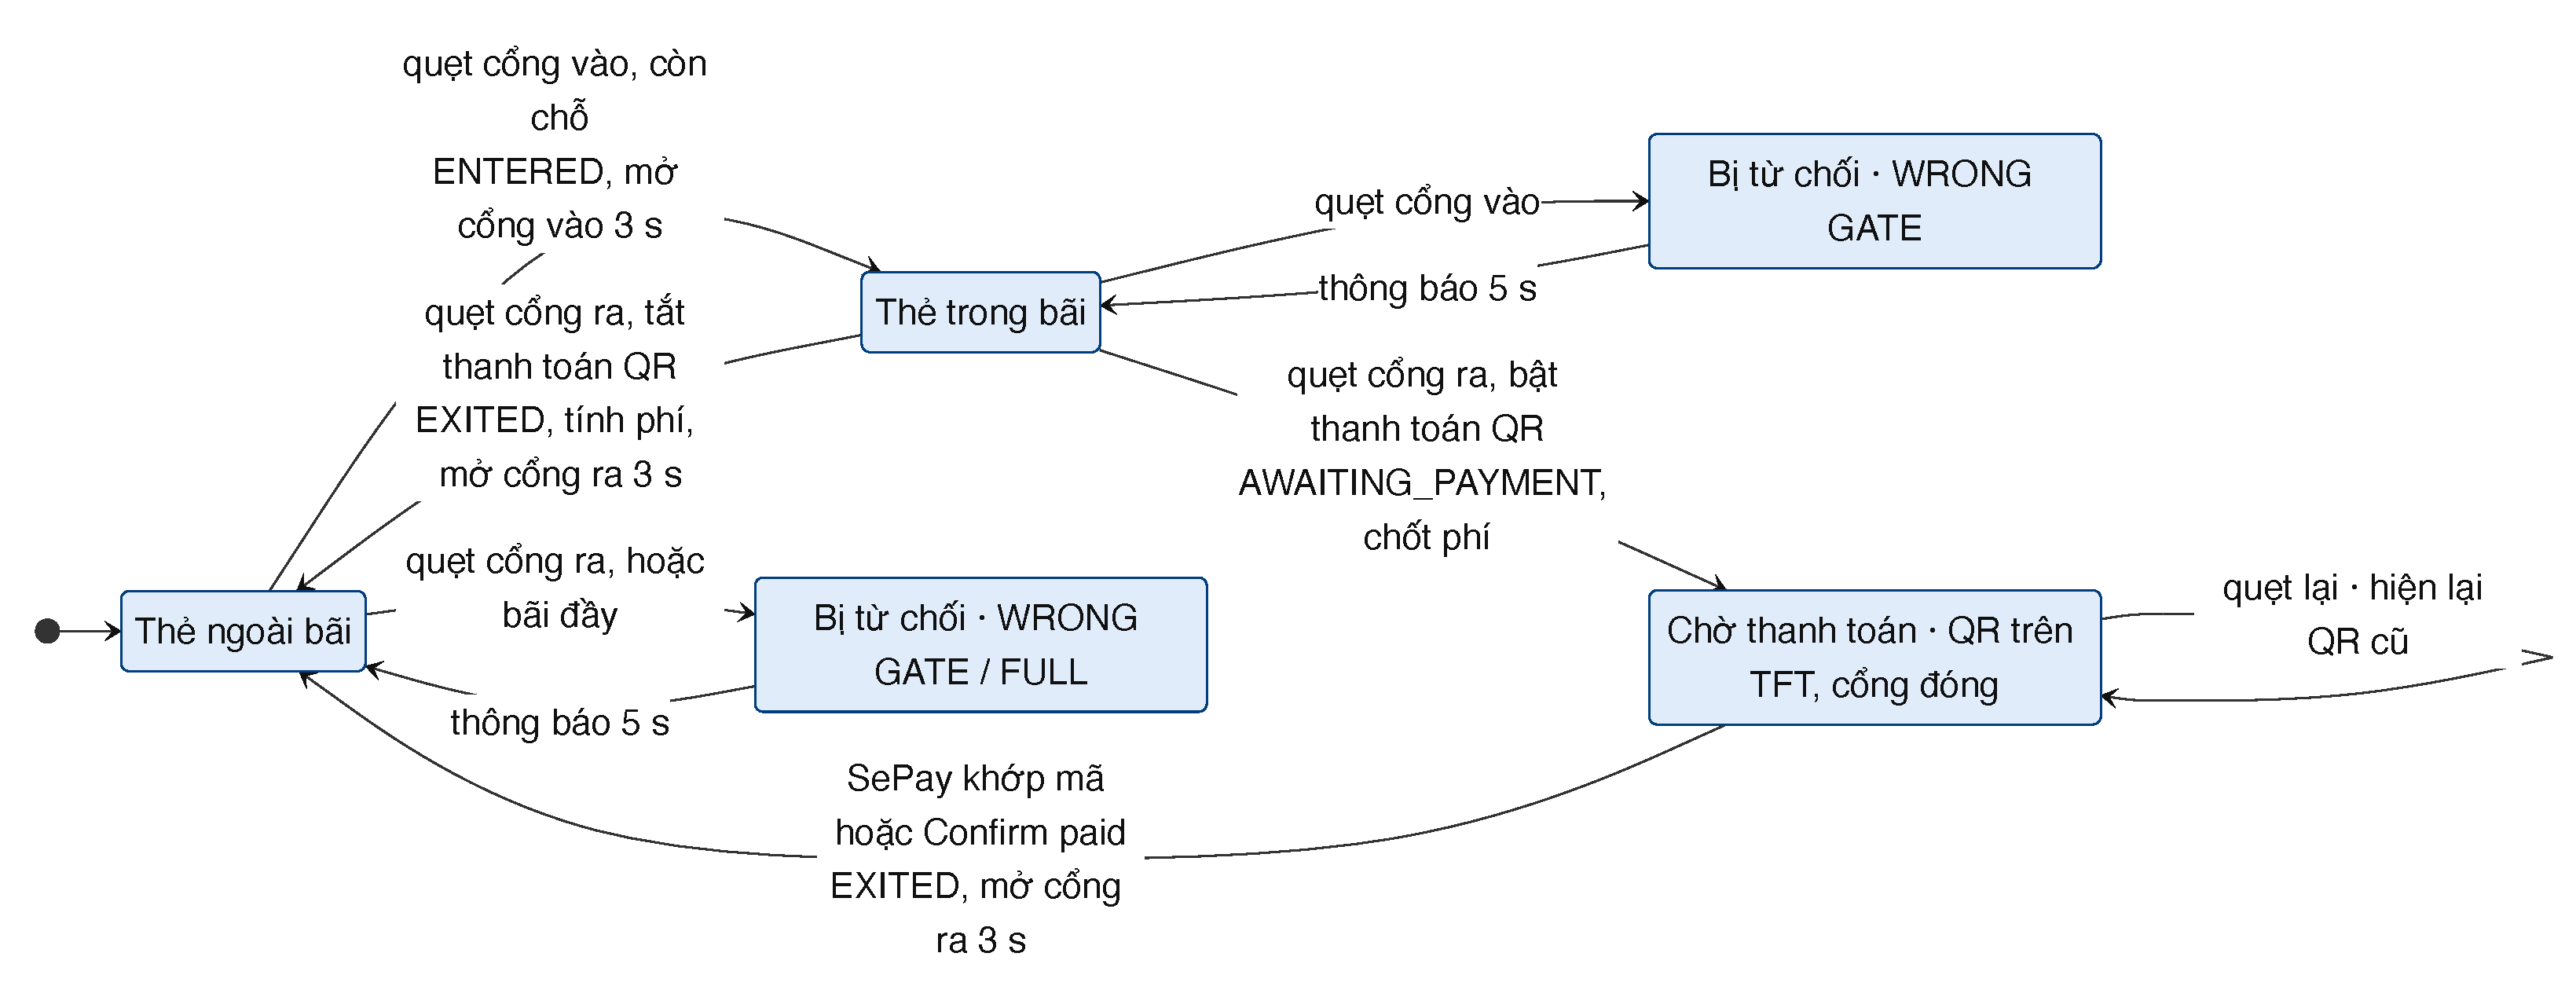
\includegraphics[width=0.92\linewidth]{fsm_card.pdf}
\vspace{6pt}
\small
\begin{columns}[T]
\column{0.32\textwidth}
\pill{ok}{VÀO} Quẹt cổng vào: mở cổng vào 3\,s, bắt đầu tính giờ
\column{0.32\textwidth}
\pill{uet}{RA} Quẹt cổng ra: tính phí, hiện mã VietQR hoặc hóa đơn
\column{0.32\textwidth}
\pill{bad}{TỪ CHỐI} Sai cổng, bãi đầy, đang ngập — báo rõ trên TFT
\end{columns}
\vspace{4pt}
\raggedright\scriptsize Phiên gửi xe lưu trong NVS: mất điện không mất xe đang gửi.
\end{frame}

% ---------------------------------------------------------------------
\begin{frame}{Thanh toán VietQR qua SePay}
\centering
\begin{tikzpicture}[font=\scriptsize,node distance=0.42cm,
  box/.style={draw=uet,fill=soft,rounded corners=3pt,align=center,minimum height=1.2cm,text width=2.2cm},
  arr/.style={-{Stealth},thick,uet}]
\node[box] (a) {\textbf{Quẹt thẻ}\\cổng ra};
\node[box,right=of a] (b) {\textbf{Máy chủ}\\tính phí, tạo mã\\VietQR trên TFT};
\node[box,right=of b] (c) {\textbf{App ngân hàng}\\quét mã,\\chuyển khoản};
\node[box,right=of c] (d) {\textbf{SePay}\\ghi nhận\\giao dịch BIDV};
\node[box,right=of d,fill=ok!15,draw=ok] (e) {\textbf{Mở cổng ra}\\hóa đơn,\\ghi doanh thu};
\draw[arr] (a)--(b); \draw[arr] (b)--(c); \draw[arr] (c)--(d); \draw[arr] (d)--(e);
\draw[arr,dashed] (b.south) to[bend right=25] node[below]{tác vụ \code{sepay} hỏi API mỗi 3\,s (HTTPS)} (d.south);
\end{tikzpicture}
\vspace{10pt}
\begin{columns}[T]
\column{0.5\textwidth}
\small
\begin{itemize}
  \item Mã theo chuẩn \textbf{NAPAS/EMVCo} (TLV + CRC16), có sẵn số tiền
  \item Nội dung chuyển khoản \code{PKxxxxxx} riêng cho từng lượt
  \item Khớp khi giao dịch chứa đúng mã \textbf{và} đủ tiền
\end{itemize}
\column{0.46\textwidth}
\small
\begin{itemize}
  \item Quá 180\,s hoặc mất Internet: người vận hành bấm \emph{Xác nhận đã trả} trên web
  \item Mỗi lúc một xe thanh toán; xe sau thấy \emph{NEXT CAR: WAIT}
  \item Số tài khoản, token: nhập qua \code{menuconfig}, không nằm trong Git
\end{itemize}
\end{columns}
\end{frame}

% ---------------------------------------------------------------------
\begin{frame}{An toàn: cháy, ngập và mất cảm biến}
\begin{columns}[T]
\column{0.32\textwidth}
\begin{block}{\bt{Cháy}}
\small
\begin{itemize}
  \item Còi kêu liên tục
  \item \textbf{Mở cả hai thanh chắn} để sơ tán
  \item TFT và web chuyển màn hình cảnh báo đỏ
\end{itemize}
\end{block}
\column{0.32\textwidth}
\begin{block}{\bt{Ngập nước}}
\small
\begin{itemize}
  \item Bật khi nước $\ge$ 20\,mm, tắt khi $\le$ 15\,mm (trễ, chống nhấp nháy)
  \item Còi kêu, \textbf{từ chối xe vào}
  \item Xe trong bãi vẫn ra được
\end{itemize}
\end{block}
\column{0.32\textwidth}
\begin{block}{\bt{Mất cảm biến}}
\small
\begin{itemize}
  \item 3\,s không có dữ liệu $\Rightarrow$ \emph{SENSOR OFFLINE}
  \item Ô đỗ chuyển xám, hiện trạng thái cuối
  \item Không coi ô cũ là còn trống
\end{itemize}
\end{block}
\end{columns}
\vspace{10pt}
\centering\small Trạng thái báo cháy được gửi ngay khi cảm biến lửa ổn định 50\,ms, không chờ chu kỳ 1\,s.
\end{frame}

% ---------------------------------------------------------------------
\begin{frame}{Giám sát: màn hình TFT và trang web}
\begin{columns}[c]
\column{0.3\textwidth}
\centering
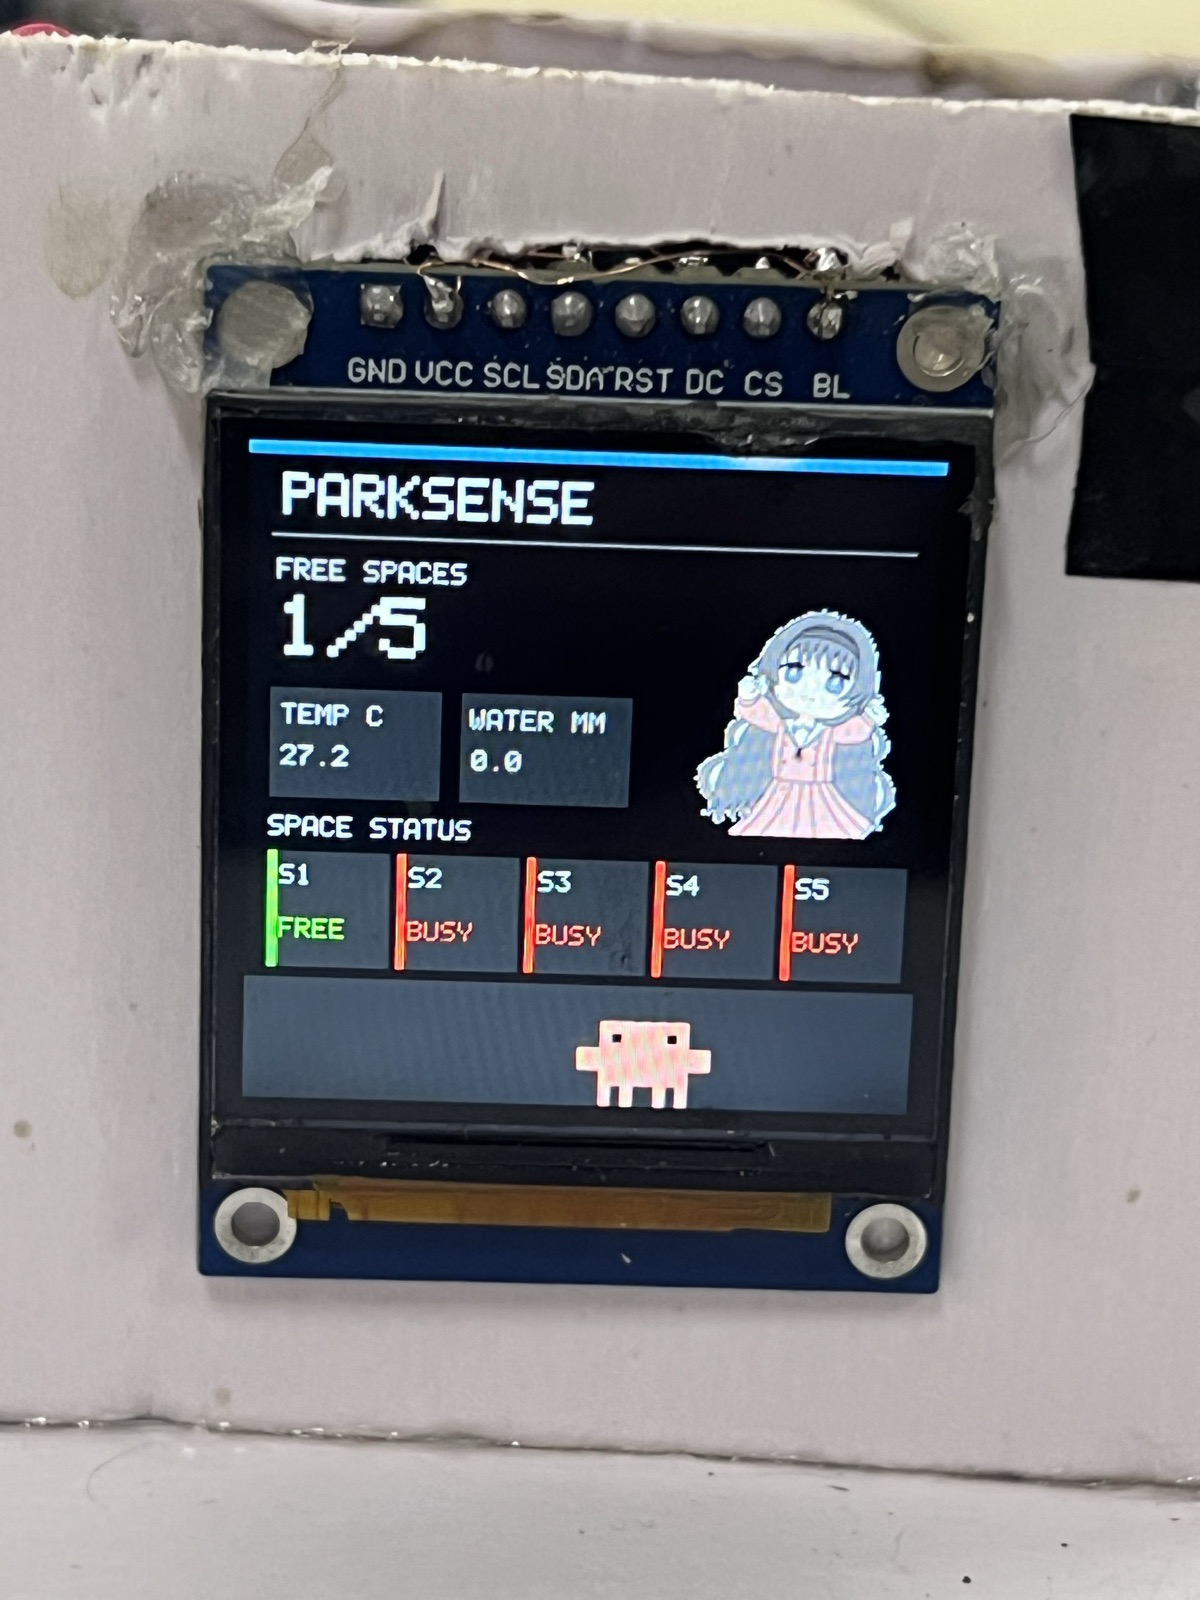
\includegraphics[height=5.6cm]{tft_live.jpg}\\[-1pt]
\scriptsize TFT tại bãi: chỗ trống, nhiệt độ, mực nước, hóa đơn
\column{0.68\textwidth}
\centering
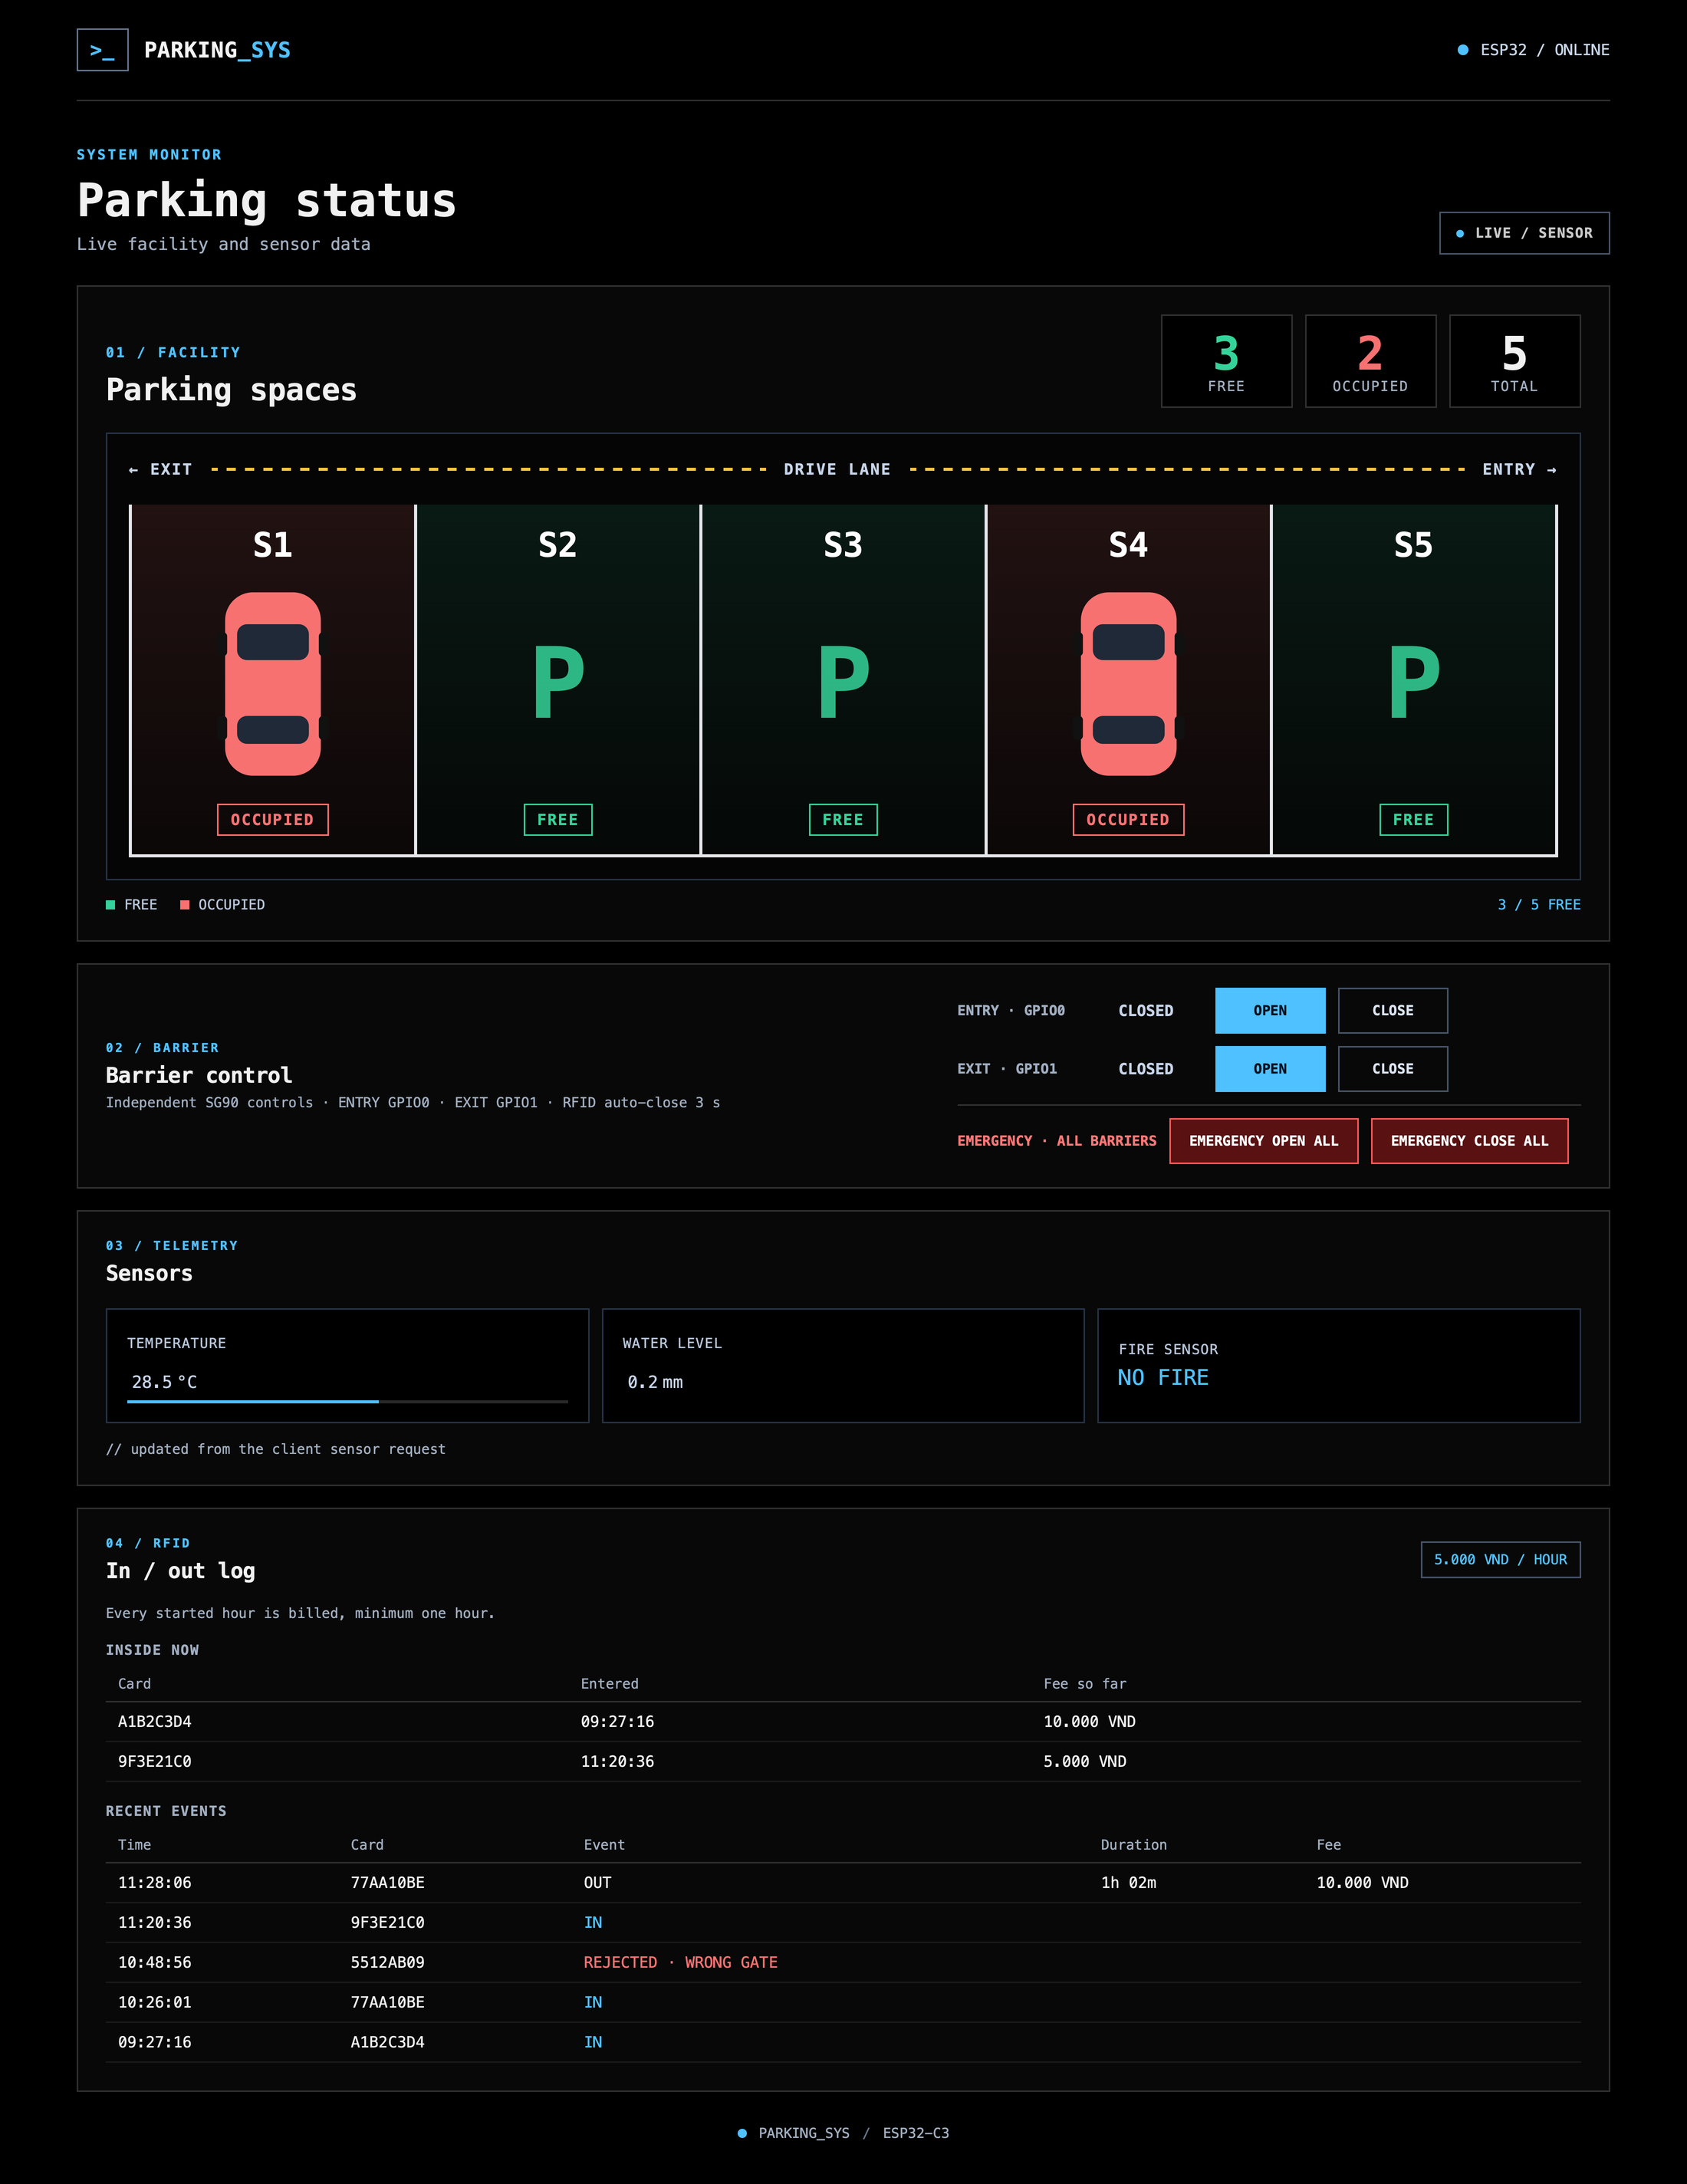
\includegraphics[height=5.6cm]{dashboard.png}\hspace{6pt}%
\begin{minipage}[c]{0.36\linewidth}\scriptsize\raggedright
\textbf{\code{parking.local}}
\begin{itemize}
  \item Sơ đồ 5 ô đỗ
  \item Mở/đóng thanh chắn (cần PIN)
  \item Cảm biến, cảnh báo
  \item Nhật ký vào/ra
  \item Doanh thu hôm nay, 7 ngày
  \item Xác nhận thanh toán
\end{itemize}
\end{minipage}
\end{columns}
\end{frame}

% ---------------------------------------------------------------------
\begin{frame}{Kiểm thử: 384 phép kiểm tra tự động}
\begin{columns}[T]
\column{0.46\textwidth}
\small
\begin{tabularx}{\linewidth}{@{}>{\raggedright\arraybackslash}Xr@{}}
\toprule
\textbf{Bộ kiểm thử} & \textbf{Số phép} \\ \midrule
\code{rfid\_session}\newline{\scriptsize phiên, phí, QR, ngập, doanh thu} & 149 \\
\code{gif\_frames} (ảnh động) & 89 \\
\code{json\_parsers} & 78 \\
\code{payment} (VietQR, SePay) & 30 \\
\code{rfid\_client} (ESP8266) & 23 \\
\code{sensor\_client} (ESP8266) & 15 \\ \midrule
\textbf{Tổng} & \textbf{384} \\
\bottomrule
\end{tabularx}
\column{0.48\textwidth}
\small
\begin{itemize}
  \item Chạy trên máy tính, không cần phần cứng: \code{make -C tests}
  \item \textbf{Lớp giả lập Arduino} để chạy nguyên mã hai sketch ESP8266
  \item Mã VietQR khớp từng byte với mẫu đã công bố (CRC \code{AB76})
  \item 27 kịch bản kiểm thử trên phần cứng (S1–S27)
\end{itemize}
\end{columns}
\end{frame}

% ---------------------------------------------------------------------
\begin{frame}{Kịch bản demo trực tiếp}
\scriptsize
\begin{tabularx}{\linewidth}{@{}c>{\raggedright\arraybackslash}p{5.4cm}>{\raggedright\arraybackslash}X@{}}
\toprule
\textbf{\#} & \textbf{Thao tác} & \textbf{Kết quả mong đợi} \\ \midrule
1 & Cấp nguồn, mở \code{http://parking.local} trên điện thoại & TFT và web hiện 5/5 chỗ trống \\
2 & Đặt xe vào ô 1 và ô 4 & Ô chuyển đỏ, còn 3/5 — TFT tức thì, web $\approx$ 1\,s \\
3 & Quẹt thẻ ở cổng \textbf{vào} & Cổng vào mở, tự đóng sau 3\,s; nhật ký ghi IN \\
4 & Quẹt lại thẻ đó ở cổng vào & \textcolor{bad}{WRONG GATE}, cổng không mở \\
5 & Quẹt thẻ ở cổng \textbf{ra} & TFT hiện mã VietQR, số tiền, mã \code{PKxxxxxx} \\
6 & Quét mã bằng app ngân hàng, chuyển khoản & Trong $\approx$ 3\,s cổng ra mở, hóa đơn, doanh thu tăng \\
7 & Đưa lửa (bật lửa) gần cảm biến lửa & Còi kêu, \textbf{cả hai cổng mở}, màn hình cảnh báo đỏ \\
8 & Nhúng cảm biến nước & Cảnh báo ngập, quẹt cổng vào bị từ chối \\
9 & Rút nguồn Sensor Client & Sau 3\,s: \emph{SENSOR OFFLINE}, ô chuyển xám \\
10 & Trên web: nhập PIN, bấm mở thanh chắn & Thanh chắn mở theo lệnh \\
\bottomrule
\end{tabularx}
\vspace{4pt}
\raggedright\scriptsize\textbf{Dự phòng:} không có Internet thì ở bước 6 bấm \emph{Xác nhận đã trả} trên web;
không có phần cứng thì chạy \code{examples/udp\_rfid\_sender.py} và \code{udp\_sender.py} để giả lập client.
\end{frame}

% ---------------------------------------------------------------------
\begin{frame}{Kết quả và hạn chế}
\begin{columns}[T]
\column{0.48\textwidth}
\begin{block}{\bt{Đạt được}}
\small
\begin{itemize}
  \item 3 bo phối hợp, \textbf{10/10 use case} hiện thực và có kiểm thử
  \item Firmware máy chủ 1,11\,MB, 31\% RAM tĩnh, còn 28\% flash ứng dụng
  \item Thanh toán VietQR tự động qua SePay
  \item Lưu phiên và doanh thu vào NVS, chịu được mất điện
\end{itemize}
\end{block}
\column{0.48\textwidth}
\begin{block}{\bt{Hạn chế còn lại}}
\small
\begin{itemize}
  \item Web dùng HTTP, UDP không ký: tin vào Wi-Fi WPA2 của nhóm
  \item Phụ thuộc router chung; router phải tắt chế độ cô lập thiết bị
  \item Token SePay nằm trong flash máy chủ
  \item Chưa có RTC: giờ lấy từ trình duyệt
\end{itemize}
\end{block}
\end{columns}
\vspace{6pt}
\small\textbf{Hướng phát triển:} cảm biến dưới thanh chắn, danh sách thẻ đăng ký, HMAC + HTTPS, RTC DS3231, MQTT lên đám mây, OTA.
\end{frame}

% ---------------------------------------------------------------------
\begin{frame}{Phân công}
\small
\begin{columns}[T]
\column{0.32\textwidth}
\begin{block}{\bt{Nguyễn Chí Minh}}
\scriptsize Phần mềm và tích hợp
\begin{itemize}
  \item Firmware máy chủ, tác vụ FreeRTOS
  \item Driver TFT, giao diện
  \item Giao thức UDP, VietQR, SePay
  \item Trang web, kiểm thử tự động
\end{itemize}
\end{block}
\column{0.32\textwidth}
\begin{block}{\bt{Đinh Đức Thịnh}}
\scriptsize Điện và phần cứng
\begin{itemize}
  \item Chọn linh kiện, so sánh vi điều khiển
  \item Thiết kế và tối ưu nguồn điện
  \item Sơ đồ chân, đi dây ba bo
  \item Firmware hai client ESP8266
\end{itemize}
\end{block}
\column{0.32\textwidth}
\begin{block}{\bt{Nguyễn Việt Tiến}}
\scriptsize Mô hình và thanh chắn
\begin{itemize}
  \item Thiết kế, dựng mô hình bãi xe
  \item Cơ cấu thanh chắn servo
  \item Firmware servo và còi
  \item Kiểm thử phần cứng, tài liệu
\end{itemize}
\end{block}
\end{columns}
\vspace{8pt}
\centering\small Mức đóng góp \textbf{ngang nhau} (33,3\% mỗi người).
\end{frame}

% ---------------------------------------------------------------------
\begin{frame}[plain]
\begin{tikzpicture}[remember picture,overlay]
  \fill[uet] (current page.south west) rectangle (current page.north east);
  \node[text=white,font=\Huge\bfseries] at ([yshift=0.6cm]current page.center) {Cảm ơn thầy và các bạn!};
  \node[text=white!80!uet,font=\large] at ([yshift=-0.5cm]current page.center) {Hỏi và đáp};
  \node[text=white!65!uet,font=\scriptsize] at ([yshift=-1.6cm]current page.center)
    {github.com/thinhdinh25/INT3108\_embedded-Smart-Parking-Project};
\end{tikzpicture}
\end{frame}

\end{document}
